%!TEX TS-program = xelatex
\documentclass[notes,12pt, aspectratio=169]{beamer}

\usepackage{amsmath,amsfonts,amssymb,amsthm,mathtools}  % пакеты для математики
\usepackage{minted}

\usepackage[english, russian]{babel} % выбор языка для документа
\usepackage[utf8]{inputenc} % задание utf8 кодировки исходного tex файла
\usepackage[X2,T2A]{fontenc}        % кодировка

\usepackage{fontspec}         % пакет для подгрузки шрифтов
\setmainfont{Helvetica}  % задаёт основной шрифт документа

% why do we need \newfontfamily:
% http://tex.stackexchange.com/questions/91507/
\newfontfamily{\cyrillicfonttt}{Helvetica}
\newfontfamily{\cyrillicfont}{Helvetica}
\newfontfamily{\cyrillicfontsf}{Helvetica}

\usepackage{unicode-math}     % пакет для установки математического шрифта
% \setmathfont{Neo Euler} % шрифт для математики

\usepackage{polyglossia}      % Пакет, который позволяет подгружать русские буквы
\setdefaultlanguage{russian}  % Основной язык документа
\setotherlanguage{english}    % Второстепенный язык документа

% Шрифт для кода
\setmonofont[Scale=0.85]{Monaco}
\usepackage{verbments}

\usepackage{pgfpages}
% These slides also contain speaker notes. You can print just the slides,
% just the notes, or both, depending on the setting below. Comment out the want
% you want.
%\setbeameroption{hide notes} % Only slide
%\setbeameroption{show only notes} % Only notes
%\setbeameroption{show notes on second screen=right} % Both

\usepackage{array}

\usepackage{tikz}
\usepackage{verbatim}
\setbeamertemplate{note page}{\pagecolor{yellow!5}\insertnote}
\usetikzlibrary{positioning}
\usetikzlibrary{snakes}
\usetikzlibrary{calc}
\usetikzlibrary{arrows}
\usetikzlibrary{decorations.markings}
\usetikzlibrary{shapes.misc}
\usetikzlibrary{matrix,shapes,arrows,fit,tikzmark}

\usepackage{hyperref}
\usepackage{lipsum}
\usepackage{multimedia}
\usepackage{multirow}
\usepackage{dcolumn}
\usepackage{bbm}
\newcolumntype{d}[0]{D{.}{.}{5}}

\usepackage{changepage}
\usepackage{appendixnumberbeamer}
\newcommand{\beginbackup}{
   \newcounter{framenumbervorappendix}
   \setcounter{framenumbervorappendix}{\value{framenumber}}
   \setbeamertemplate{footline}
   {
     \leavevmode%
     \hline
     box{%
       \begin{beamercolorbox}[wd=\paperwidth,ht=2.25ex,dp=1ex,right]{footlinecolor}%
%         \insertframenumber  \hspace*{2ex} 
       \end{beamercolorbox}}%
     \vskip0pt%
   }
 }
\newcommand{\backupend}{
   \addtocounter{framenumbervorappendix}{-\value{framenumber}}
   \addtocounter{framenumber}{\value{framenumbervorappendix}} 
}

% для имитации питоновского синтаксиса 
\newcommand{\pgr}[1]{{\color{green} \textbf{#1}}}


%%%%%%%%%% Работа с картинками %%%%%%%%%
\usepackage{graphicx}                  % Для вставки рисунков
\usepackage{graphics}
\graphicspath{{images_1/}}    % можно указать папки с картинками
\usepackage{wrapfig}                   % Обтекание рисунков и таблиц текстом

\usepackage[space]{grffile}
\usepackage{booktabs}

% These are my colors -- there are many like them, but these ones are mine.
\definecolor{blue}{RGB}{0,114,178}
\definecolor{red}{RGB}{213,94,0}
\definecolor{yellow}{RGB}{240,228,66}
\definecolor{green}{RGB}{0,128, 0}

\hypersetup{
  colorlinks=false,
  linkbordercolor = {white},
  linkcolor = {blue}
}


%% I use a beige off white for my background
\definecolor{MyBackground}{RGB}{255,253,218}

%% Uncomment this if you want to change the background color to something else
%\setbeamercolor{background canvas}{bg=MyBackground}

%% Change the bg color to adjust your transition slide background color!
\newenvironment{transitionframe}{
  \setbeamercolor{background canvas}{bg=yellow}
  \begin{frame}}{
    \end{frame}
}

\setbeamercolor{frametitle}{fg=blue}
\setbeamercolor{title}{fg=black}
\setbeamertemplate{footline}[frame number]
\setbeamertemplate{navigation symbols}{} 
\setbeamertemplate{itemize items}{-}
\setbeamercolor{itemize item}{fg=blue}
\setbeamercolor{itemize subitem}{fg=blue}
\setbeamercolor{enumerate item}{fg=blue}
\setbeamercolor{enumerate subitem}{fg=blue}
\setbeamercolor{button}{bg=MyBackground,fg=blue,}


% If you like road maps, rather than having clutter at the top, have a roadmap show up at the end of each section 
% (and after your introduction)
% Uncomment this is if you want the roadmap!
% \AtBeginSection[]
% {
%    \begin{frame}
%        \frametitle{Roadmap of Talk}
%        \tableofcontents[currentsection]
%    \end{frame}
% }
\setbeamercolor{section in toc}{fg=blue}
\setbeamercolor{subsection in toc}{fg=red}
\setbeamersize{text margin left=1em,text margin right=1em} 

% списки, которые растягиваются на всю величину слайда 
\newenvironment{wideitemize}{\itemize\addtolength{\itemsep}{10pt}}{\enditemize}



\title[]{\textcolor{blue}{Практический анализ данных и машинное обучение: искусственные нейронные сети}}
\author{Ульянкин Филипп}
\date{\today}


\begin{document}

%%% TIKZ STUFF
\tikzset{   
        every picture/.style={remember picture,baseline},
        every node/.style={anchor=base,align=center,outer sep=1.5pt},
        every path/.style={thick},
        }
\newcommand\marktopleft[1]{%
    \tikz[overlay,remember picture] 
        \node (marker-#1-a) at (-.3em,.3em) {};%
}
\newcommand\markbottomright[2]{%
    \tikz[overlay,remember picture] 
        \node (marker-#1-b) at (0em,0em) {};%
}
\tikzstyle{every picture}+=[remember picture] 
\tikzstyle{mybox} =[draw=black, very thick, rectangle, inner sep=10pt, inner ysep=20pt]
\tikzstyle{fancytitle} =[draw=black,fill=red, text=white]
%%%% END TIKZ STUFF

% Title Slide
\begin{frame}
\maketitle
\centering Введение в Нейросети
\end{frame}


{
	\usebackgroundtemplate{ 
	\hspace{3cm}	
\includegraphics[height=\paperheight]{ya.jpg}}
\begin{frame}
\end{frame}
}


\begin{frame}{Agenda}
\begin{wideitemize}

\item Немного истории

\item Всё, что вы хотели знать о градиентном спуске, но боялись спросить

\item Перцептрон

\item Алгоритм обратного распространения ошибки, учим нейросеть руками

\item Нейросети  — конструктор Lego 

\end{wideitemize} 
\end{frame}


\begin{transitionframe}
	\begin{center}
		\Huge Немного истории
	\end{center}
\end{transitionframe}


\begin{frame}
\begin{center}
	\resizebox{0.51\linewidth}{!}{
		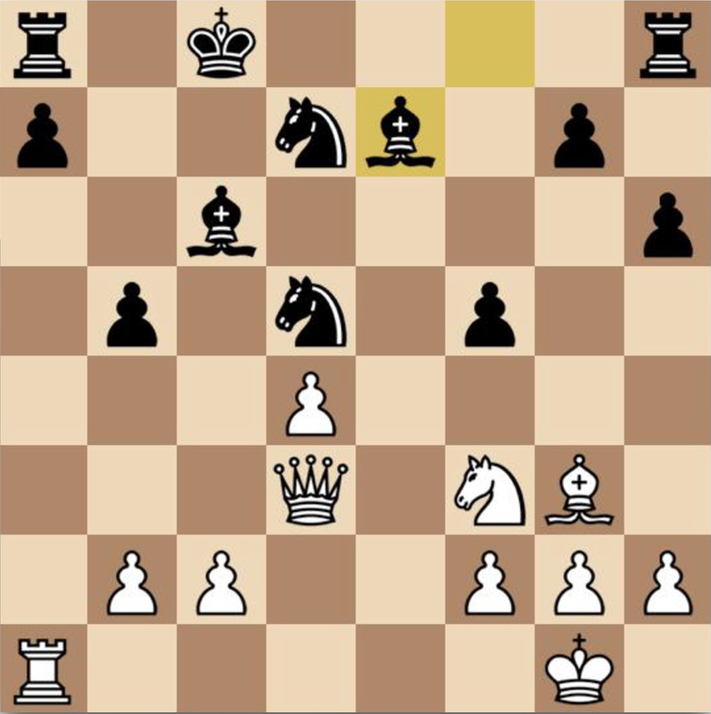
\includegraphics{chess_1.png}
	}
\end{center}
\end{frame}


\begin{frame}
\begin{center}
	\resizebox{0.51\linewidth}{!}{
		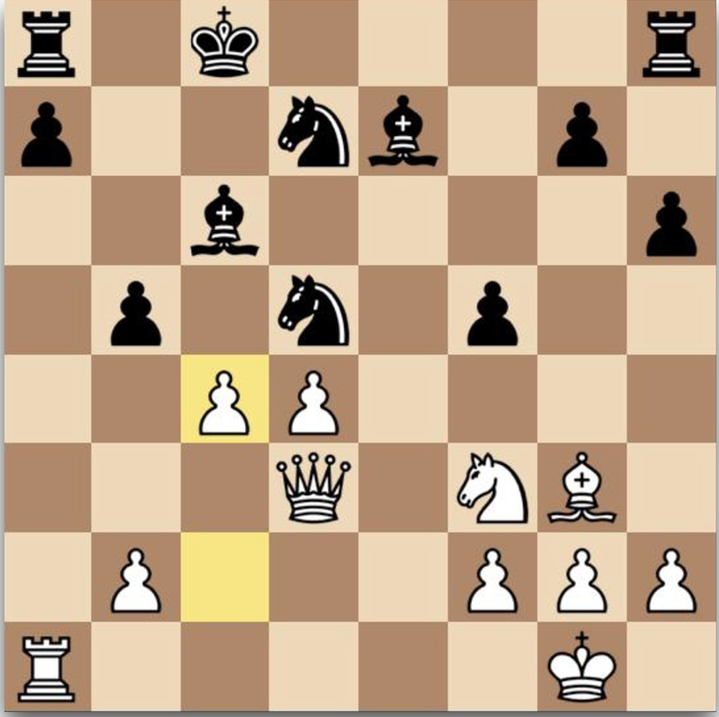
\includegraphics{chess_2.png}
	}
\end{center}
\end{frame}


\begin{frame}{ }
\begin{columns}[T]
\begin{column}{.49\textwidth}
	\hspace{1.5cm}
	\resizebox{0.51\linewidth}{!}{
	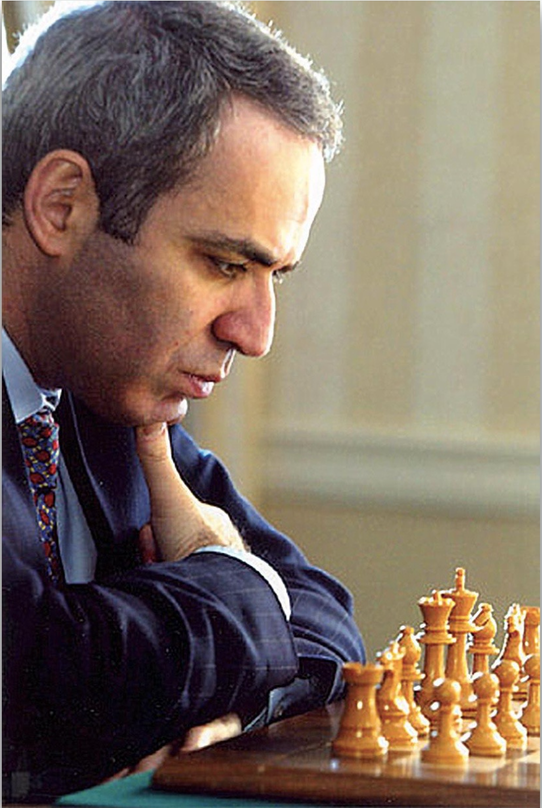
\includegraphics{kasparov.png}
}
\mbox{ }

\hspace{1.9cm} Garry Kasparov
\end{column}
\hfill
\begin{column}{.49\textwidth}
%%% 
\end{column}
\end{columns}
\end{frame}


\begin{frame}
\begin{columns}[T]
	\begin{column}{.49\textwidth}
		\hspace{1.5cm}
		\resizebox{0.51\linewidth}{!}{
			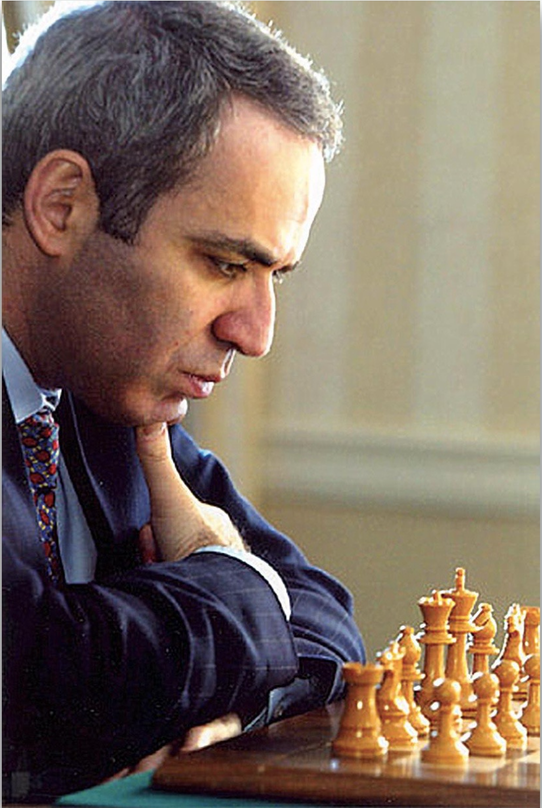
\includegraphics{kasparov.png}
		}
		\mbox{ }
		
		\hspace{1.9cm} Garry Kasparov
	\end{column}
	\hfill
	\begin{column}{.49\textwidth}
	\hspace{1.5cm}
	\resizebox{0.51\linewidth}{!}{
		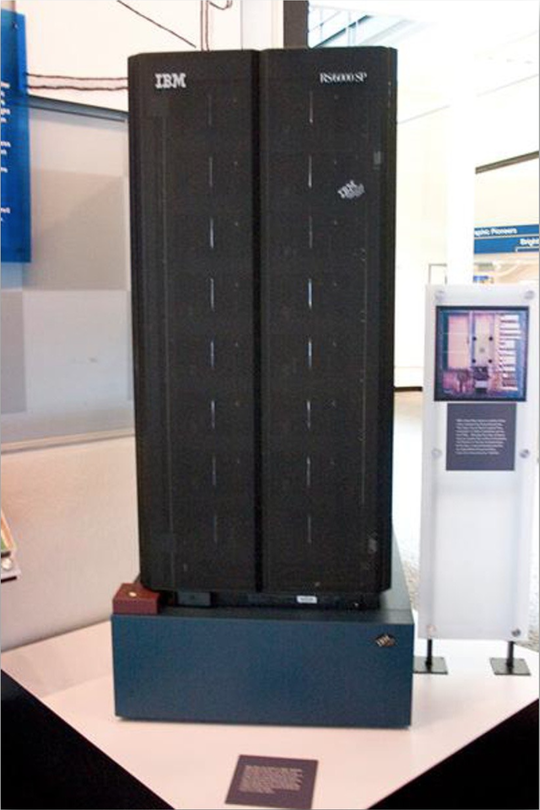
\includegraphics{deepblue.png}
	}
	\mbox{ }
	
	\hspace{2.5cm} Deepblue
	\end{column}
\end{columns}
\end{frame}


\begin{frame}
\begin{center}
	\resizebox{0.4\linewidth}{!}{
		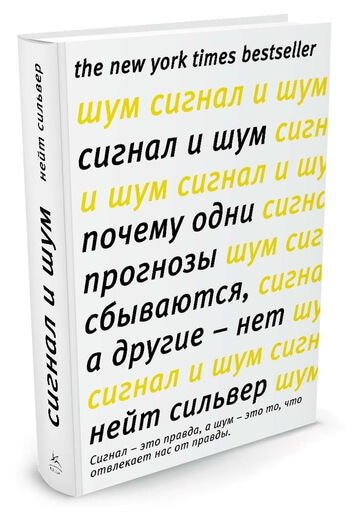
\includegraphics{signal.jpg}
	}
\end{center}
\end{frame}


\begin{frame}
\begin{wideitemize}
	\item Шашки полностью решены в 2007 году 
	\item Шахматы: впервые компьютер побеждает человека в феврале 1996 года 
	\item Шахматы: в ноябре 2005 человек в последний раз побеждает у компьютера
	\item Го: последний оплот человечества до апреля 2016 года
\end{wideitemize} 
\end{frame}

\begin{frame}{GO пал со счётом 4 : 1}
\begin{columns}[T]
	\begin{column}{.49\textwidth}
		\hspace{1.5cm}
		\resizebox{0.51\linewidth}{!}{
			
\includegraphics{alphago.png} 
		} 
		\mbox{ }
		
		\hspace{1.6cm} AlphaGo by Google
	\end{column}
	\hfill
	\begin{column}{.49\textwidth}
		\hspace{1.5cm}
		\resizebox{0.51\linewidth}{!}{
			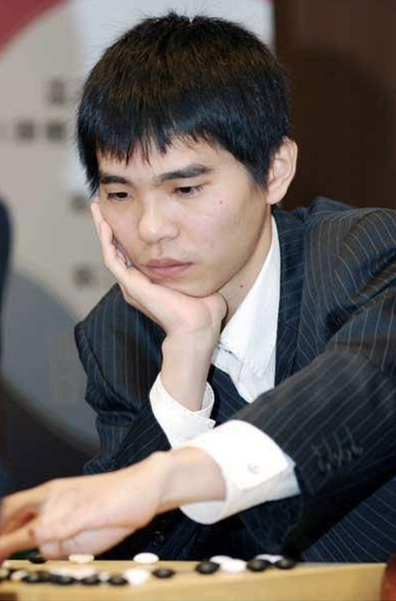
\includegraphics{lee_sedol.png}
		}
		\mbox{ }
		
		\hspace{2.5cm} Lee Sedol
	\end{column}
\end{columns}
\end{frame}

\begin{frame}
\begin{center}
	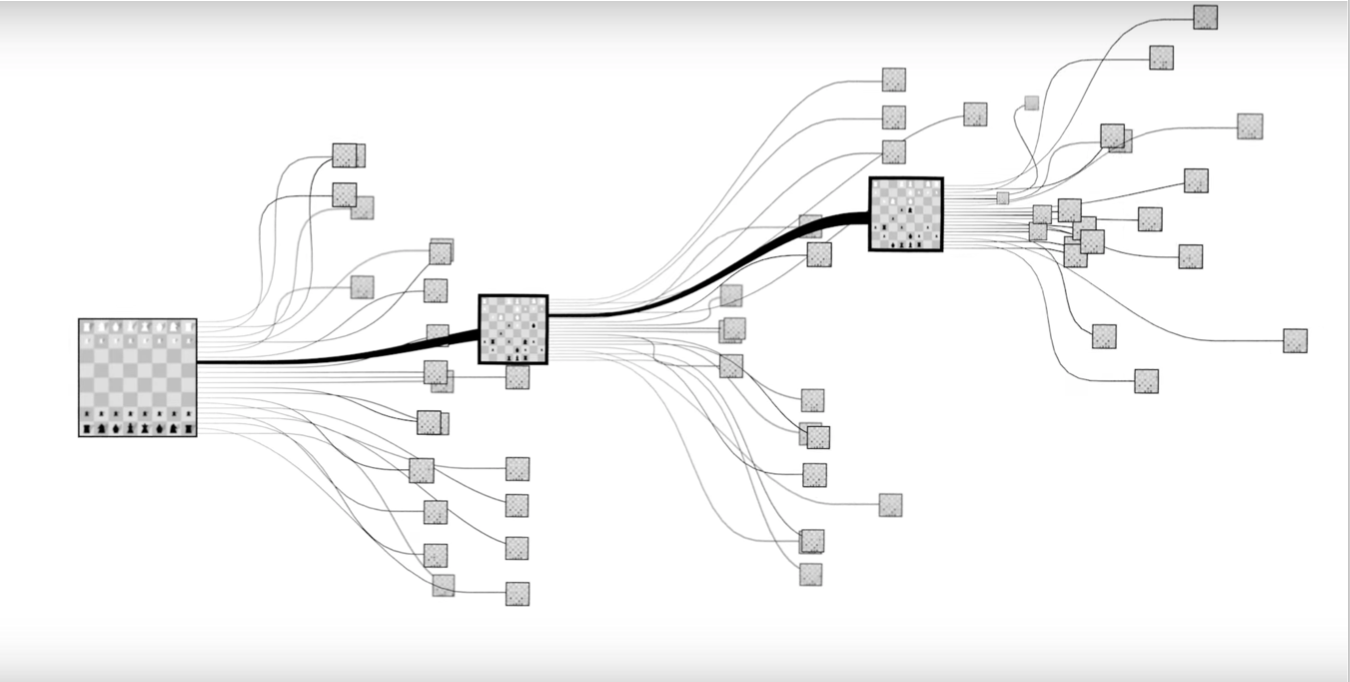
\includegraphics[width=.9\linewidth]{chees_3.png}
\end{center}
\end{frame}


\begin{frame}
\begin{center}
	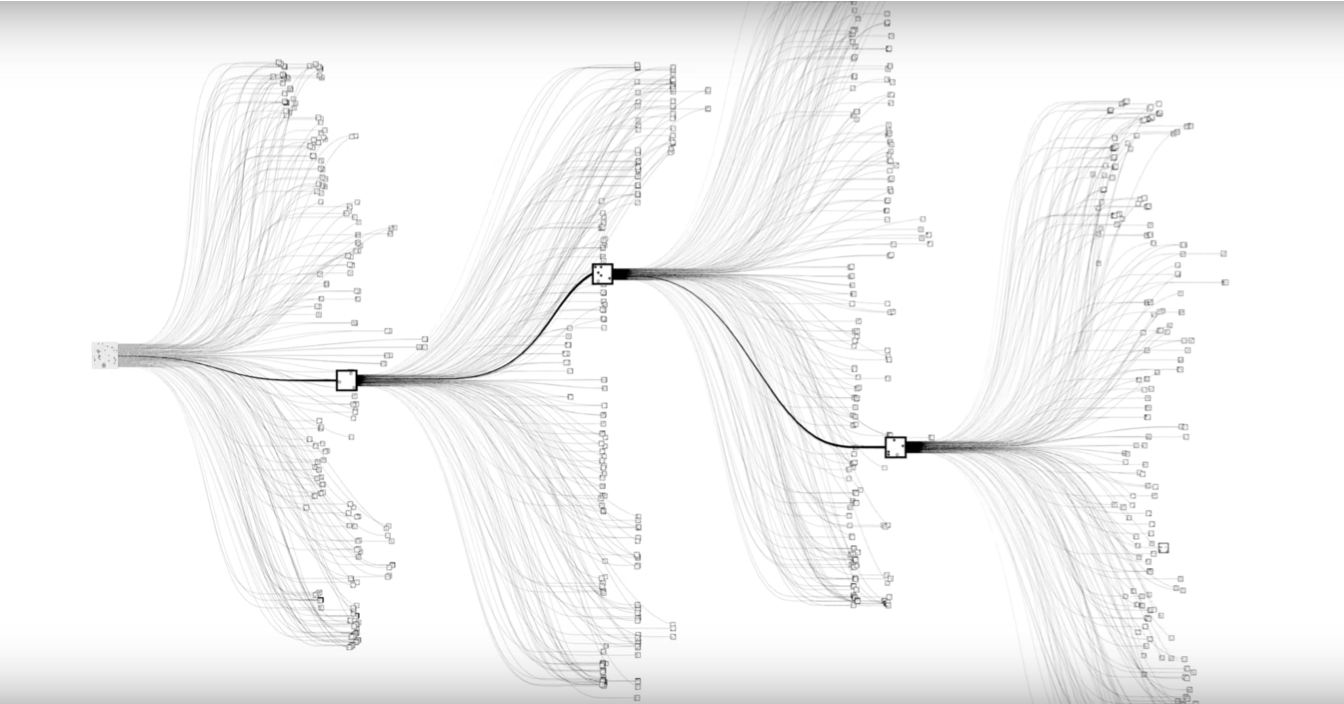
\includegraphics[width=.9\linewidth]{chess_4.png}
\end{center}
\end{frame}


\begin{frame}{О том как всё начиналось}
\begin{wideitemize}
	
	\item<1->  Середина $1950$-х — перцептрон Розенблата 
	
	\item<2-> $1956$ год — Дартмутский семинар, безграничный оптимизм
	
	\item<3->  Конец $1960$-х — провал крупного проекта по машинному переводу, первая зима 
	
	\item<4-> Начало $1980-$х —  разработан backpropagation, появление огромного числа архитектур, ренессанс нейросетей 
	
	\item<5->  Начало $1990$-х — завышенные ожидания снова не оправданы, вторая зима
	
\end{wideitemize}
\end{frame}


\begin{frame}{О том как всё начиналось}
\begin{wideitemize}
\item<1-> Середина $2000$-х — третий и единственный успешный ренессанс нейронных сеток, люди научились обучать глубокие нейросети 

\item<2-> Начиная с $2014$ года несколько архитектур друг за другом рвут ImageNet

\item<3-> Человечество копит в течение $2000$-х годов огромное количество данных, а мощности компьютеров выходят на новые рубежи
\end{wideitemize}
\end{frame}




\begin{transitionframe}
	\begin{center}
		\Huge Линейные модели
	\end{center}
\end{transitionframe}




\begin{frame}{Как обучать?}
\begin{wideitemize}
	\item «Тренировка» — поиск оптимальных $W$ и $b$
	\item «Оптимальных» — минимизирующих какой-то функционал 
	\item Какими бывают функционалы: MSE, MAE, Logloss
	\item Как оптимизировать: градиентный спуск! 
\end{wideitemize} 
\end{frame}


\begin{transitionframe}
	\begin{center}
		\Huge Градиентный спуск
	\end{center}
\end{transitionframe}


\begin{frame}[fragile]{Градиентный спуск (GD)}
Проблема оптимизации: 

\[   
L(w) = \sum_{i=1}^n L(w, x_i, y_i) \to \min_{w}
\]

Инициализация $w_0$ 
\mint{python}{while True:}
\hspace{15pt} $g_t = \frac{1}{n}\sum_{i=1}^n  \nabla L(w, x_i, y_i)$ \\
\pgr{\hspace{15pt}} $w_t = w _{t-1} - \eta_t \cdot g_t $ \\
\pgr{\hspace{15pt} if} $||w_t - w_{t-1}|| < \varepsilon:$ \\
\pgr{\hspace{30pt} break}
\end{frame}


\begin{frame}{Градиентный спуск}
\begin{center}
	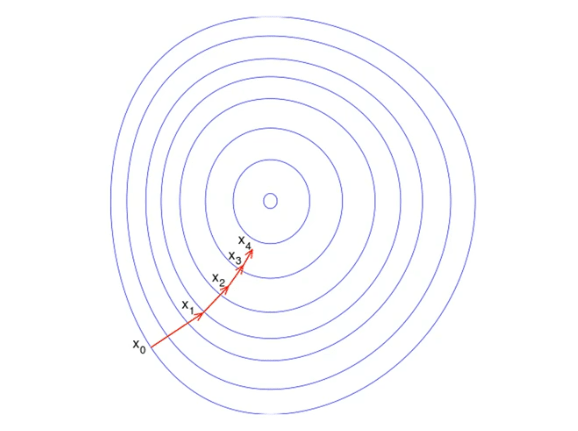
\includegraphics[width=.6\linewidth]{2dgrad.png}
\end{center}
\end{frame}


\begin{frame}[fragile]{Стохастический градиентный спуск (SGD)}
Проблема оптимизации: 

\[   
L(w) = \sum_{i=1}^n L(w, x_i, y_i) \to \min_{w}
\]


Инициализация $w_0$ 
\mint{python}{while True:}
\hspace{15pt} рандомно выбрали $i$ \\
\pgr{\hspace{15pt}} $g_t = \nabla L(w_{t-1}, x_i, y_i)$ \\
\pgr{\hspace{15pt}} $w_t = w _{t-1} - \eta_t \cdot g_t  $ \\
\pgr{\hspace{15pt} if} $||w_t - w_{t-1}|| < \varepsilon:$ \\
\pgr{\hspace{30pt} break}
\end{frame}


\begin{frame}{Стохастический градиентный спуск (SGD)}
\begin{columns}[T] %
	\begin{column}{.4\textwidth}
		\resizebox{0.95\linewidth}{!}{
			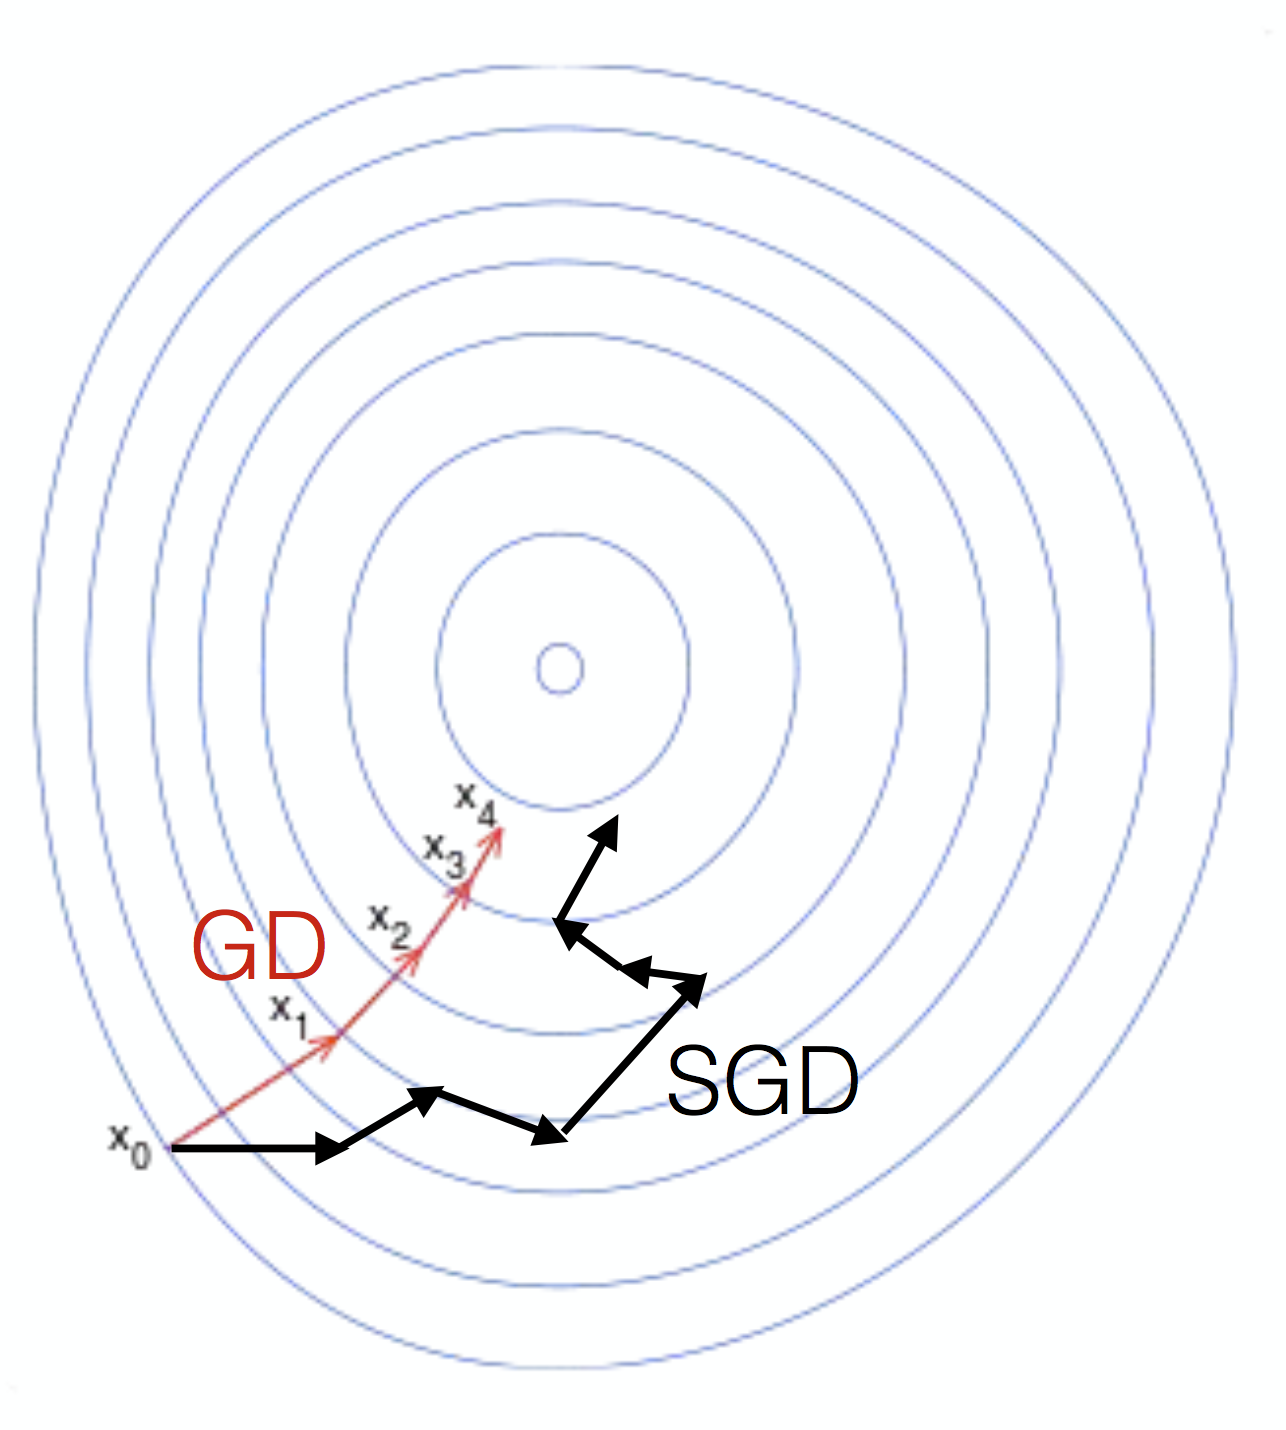
\includegraphics{st2grad.png}
		}
	\end{column}%
	\hfill%
	\begin{column}{.6\textwidth}
		\begin{wideitemize}
			\item И для GD и для SGD нет гарантий глобального минимума, сходимости
			\item SGD быстрее,на каждой итерации используется только одно наблюдение
			\item Для SGD спуск очень зашумлён 
			\item  GD: $O(n)$, SGD: $O(1)$
			\item Скорость обучения надо подбирать аккуратно, если она будет большой, мы можем скакать вокруг минимума, если маленькой - вечно ползти к нему
		\end{wideitemize}
	\end{column}%
\end{columns}
\end{frame}


\begin{frame}[fragile]{Mini-bath SGD}
Проблема оптимизации: 

\[   
L(w) = \sum_{i=1}^n L(w, x_i, y_i) \to \min_{w}
\]

Инициализация $w_0$ 
\mint{python}{while True:}
\pgr{\hspace{15pt}} рандомно выбрали $m < n$ индексов \\
\pgr{\hspace{15pt}} $g_t =\frac{1}{m}\sum_{i=1}^m  \nabla L(w, x_i, y_i)$ \\
\pgr{\hspace{15pt}} $w_t = w _{t-1} - \eta_t \cdot g_t   $ \\
\pgr{\hspace{15pt} if} $||w_t - w_{t-1}|| < \varepsilon:$ \\
\pgr{\hspace{30pt} break}
\end{frame}


\begin{frame}{Momentum SGD}

Мы считали на каждом шаге градиент по формуле  \[g_t =\frac{1}{m}\sum_{i=1}^m  \nabla L(w, x_i, y_i).\] После шага мы забывали его. {\color{red} А давайте попробуем помнить направление:} 

\begin{equation*}
	\begin{aligned}
	h_t &= \alpha \cdot h_{t-1} + \eta_t \cdot g_t \\
	w_t &= w_{t-1} - h_t
	\end{aligned}	
\end{equation*}

\begin{itemize}
	\item Движение поддерживается в том же направлении, что и на предыдущем шаге
	\item Нет резких изменений направления движения.
	\item Обычно $\alpha = 0.9$.
\end{itemize}
\end{frame}


\begin{frame}{Momentum SGD}
\begin{wideitemize}
	\item Бежим с горки и всё больше ускоряемся в том направлении, в котором были направлены сразу несколько предыдущих градиентов, но при этом движемся медленно там, где градиент постоянно меняется
	\item Хотелось бы не просто бежать с горы, но и хотя бы на полшага смотреть себе под ноги, чтобы внезапно не споткнуться $\Rightarrow$ давайте смотреть на градиент в будущей точке
	\item Согласно методу моментов $\alpha h_{t-1}$ точно будет использоваться при шаге, давайте искать $\nabla L(w_{t-1} - \alpha \cdot h_{t-1})$.
\end{wideitemize}
\end{frame}


\begin{frame}{Nesterov Momentum SGD}
\begin{center}
	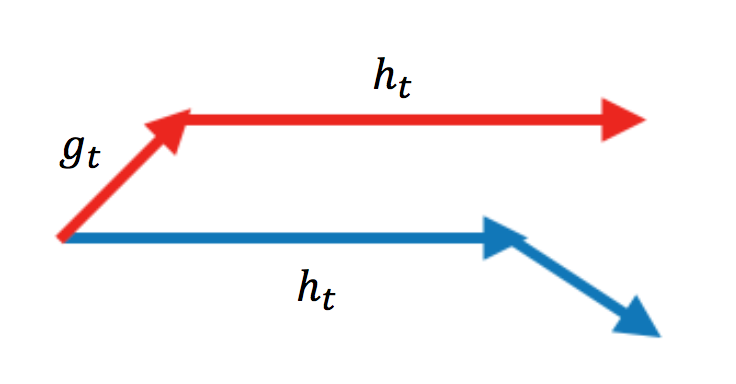
\includegraphics[width=.4\linewidth]{nesterov.png}
\end{center}

\begin{equation*}
\begin{aligned}
h_t &= \alpha \cdot h_{t-1} + \eta_t \nabla L(w_{t-1} - \alpha \cdot h_{t-1}) \\
w_t &= w_{t-1} - h_t
\end{aligned}	
\end{equation*}
\end{frame}


\begin{frame}{Momentum SGD}
\begin{wideitemize}
	\item Может сложиться, что некоторые веса уже близки к своим локальным минимумам, по этим координатам надо двигаться медленнее, а по другим быстрее $\Rightarrow$ {\color{red} адаптивные методы градиентного спуска }

	\item Шаг изменения должен быть меньше у тех параметров, которые в большей степени варьируются в данных, и больше у тех, которые менее изменчивы 
\end{wideitemize}
\end{frame}


\begin{frame}{AdaGrad}
\begin{equation*}
\begin{aligned}
G_t^j &= G_{t-1}^j + g_{tj}^2 \\
w_t^j &= w_{t-1}^j - \frac{\eta_t}{\sqrt{G_t^j + \varepsilon}} \cdot g_t^j
\end{aligned}	
\end{equation*}

\begin{itemize}
	\item  $g_t^j$ — градиент по $j-$ому параметру
	\item своя скорость обучения для каждого параметра
	\item обычно $\eta_t = 0.01$, этот параметр не имеет значения
	\item $G_t^j$ всегда увеличивается, из-за этого обучение может рано останавливаться
\end{itemize}
\end{frame}


\begin{frame}{RMSprop}
\begin{equation*}
\begin{aligned}
G_t^j &= \alpha \cdot G_{t-1}^j + (1 - \alpha) \cdot g_{tj}^2 \\
w_t^j &= w_{t-1}^j - \frac{\eta_t}{\sqrt{G_t^j + \varepsilon}} \cdot g_t^j
\end{aligned}	
\end{equation*}

\begin{itemize}
	\item Обычно $ \alpha = 0.9$
	\item Скорость обучения адаптируется к последнему сделанному шагу
\end{itemize}
\end{frame}


\begin{frame}{Adam}
\begin{equation*}
\begin{aligned}
h_t^j &= \beta_1 \cdot h_{t-1}^j + (1 - \beta_1) \cdot g_{tj} \\
G_t^j &= \beta_2 \cdot G_{t-1}^j + (1 - \beta_2) \cdot g_{tj}^2 \\
w_t^j &= w_{t-1}^j - \frac{\eta_t}{\sqrt{G_t^j + \varepsilon}} \cdot h_t^j
\end{aligned}	
\end{equation*}

\begin{itemize} 
Комбинируем momentum и индивидуальные скорости обучения
\end{itemize}
\end{frame}


\begin{frame}{Подведём итоги}
\begin{wideitemize}
	\item Momentum SGD сохраняет направление шага и позволяет добиваться более быстрой сходимости
	
	\item  Адаптивные методы позволяют находить индивидуальную скорость обучения для каждого параметра
	
	\item Adam комбинирует в себе оба подхода
\end{wideitemize}
\end{frame}


\begin{transitionframe}
	\begin{center}
		\Huge Перцептрон 
	\end{center}
\end{transitionframe}


\begin{frame}{Перцептрон}
\begin{itemize}
	\item  {\color{blue} Перцептрон —} древняя штука, придуманная Розенблатом в $1950$-е годы.
\end{itemize}
\end{frame}


\begin{frame}{Перцептрон}
\begin{center}
	\begin{tikzpicture}[line cap=round,line join=round,x=1.0cm,y=1.0cm, scale=0.45]
	\clip(-6.6,-2.6) rectangle (12.5,8);
	\fill[line width=2.pt,color=blue,fill=blue,fill opacity=0.1] (1.,4.) -- (1.,2.) -- (5.,2.) -- (5.,4.) -- cycle;
	\draw [line width=2.pt] (-3.,3.) circle (1.cm);
	\draw [line width=2.pt] (-3.,7.) circle (1.cm);
	\draw [line width=2.pt] (-3.,-1.) circle (1.cm);
	\draw [line width=2.pt,color=blue] (1.,4.)-- (1.,2.);
	\draw [line width=2.pt,color=blue] (1.,2.)-- (5.,2.);
	\draw [line width=2.pt,color=blue] (5.,2.)-- (5.,4.);
	\draw [line width=2.pt,color=blue] (5.,4.)-- (1.,4.);
	\draw [line width=2.pt] (2.9881440090657487,7.0008060081686905) circle (0.9849655397676651cm);
	\draw [line width=2.pt] (9.01246812438894,2.992225323067729) circle (0.991601954541948cm);
	\draw [->,line width=2.pt] (-2.13816854826612,6.4928052161129095) -- (1.,3.4045364792495425);
	\draw [->,line width=2.pt] (-2.000475444752397,2.969167169168543) -- (1.,2.923506797037427);
	\draw [->,line width=2.pt] (-2.16210927631272,-0.4541619881697446) -- (1.,2.5111956408556138);
	\draw [->,line width=2.pt] (2.9444109347047998,6.016811835047352) -- (2.9652378337223144,4.);
	\draw [->,line width=2.pt] (5.118418316005128,2.923506797037427) -- (8.02306241164538,2.926264942218159);
	\draw (-3.8,7.5) node[anchor=north west] {$x_1$};
	\draw (-3.8,3.5) node[anchor=north west] {$x_2$};
	\draw (-3.8,-0.5) node[anchor=north west] {$x_n$};
	\draw (3.1,5.8) node[anchor=north west] {$b$};
	\draw (2.3,7.7) node[anchor=north west] {$1$};
	\draw (8.3,3.6) node[anchor=north west] {$y$};
	\draw (-0.5,6.3) node[anchor=north west] {$w_1$};
	\draw (-1.5,4.5) node[anchor=north west] {$w_2$};
	\draw (-0.8 ,1.2) node[anchor=north west] {$w_n$};
	\draw (-3.8,1.5) node[anchor=north west] {$\mathbf{...}$};
	\draw (1.8,3.8) node[anchor=north west] {$f(z)$};
	\end{tikzpicture}
\end{center}

\begin{equation*}
\begin{aligned}
y &= f(b + w_1 \cdot x_1 + \ldots + w_n \cdot x_n) = f(X \cdot W_1) \\ 
h & = X \cdot W_1
\end{aligned}
\end{equation*}
\end{frame}


\begin{frame}{Некоторые модели — частный случай перцептрона}

\begin{wideitemize}
	\item Для регрессии возьмём $f(z) = z$.
	\item Для логистической регрессии возьмём $f(z) = \frac{1}{1 + e^{-z}}$.
\end{wideitemize}
\end{frame}




\begin{frame}{Скрытый слой}

\begin{center}
	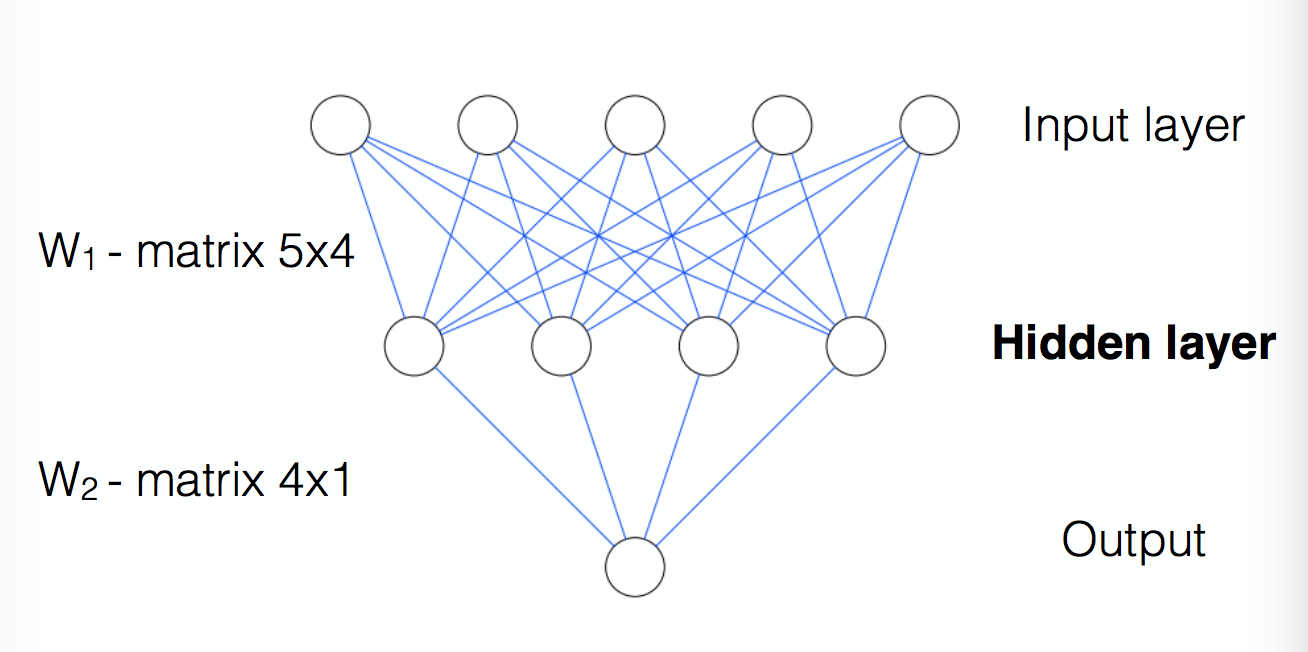
\includegraphics[width=.6\linewidth]{nn3.png}
\end{center}

\begin{equation*}
\begin{aligned}
h &= f(X \cdot W_1)\\
\hat y &= h \cdot W_2 \\
\end{aligned}
\end{equation*}
\end{frame}


\begin{frame}{Линейная активация}
\begin{center}
	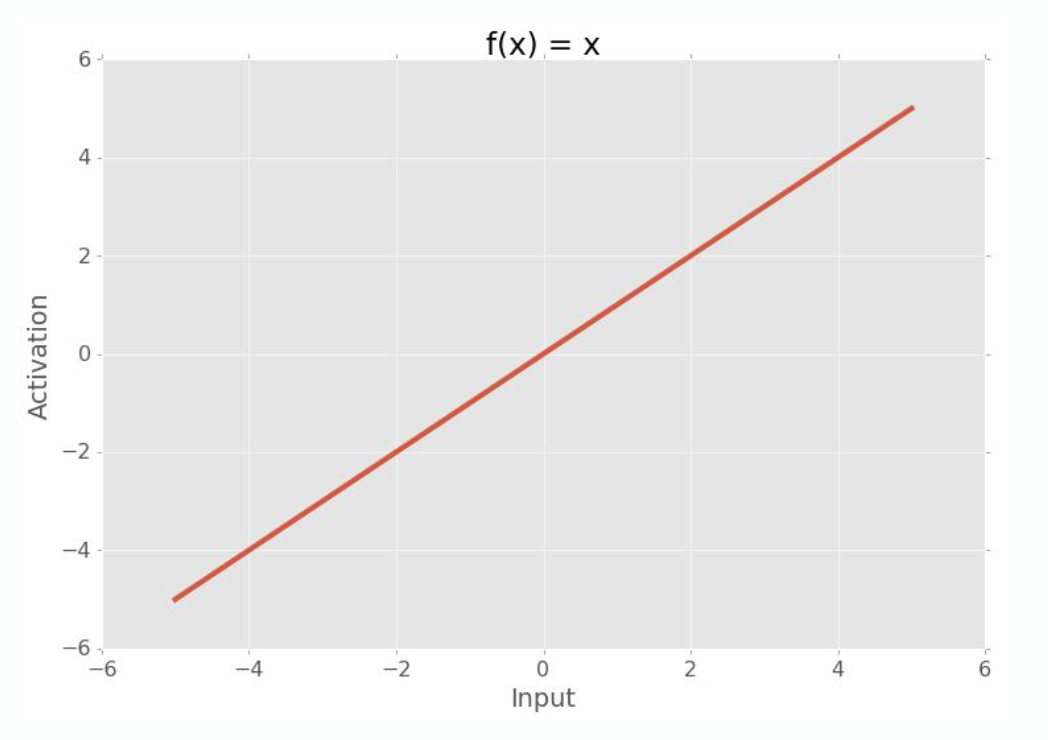
\includegraphics[width=.4\linewidth]{linear_activation.png}
\end{center}
\end{frame}


\begin{frame}{Линейная активация}
\begin{center}
	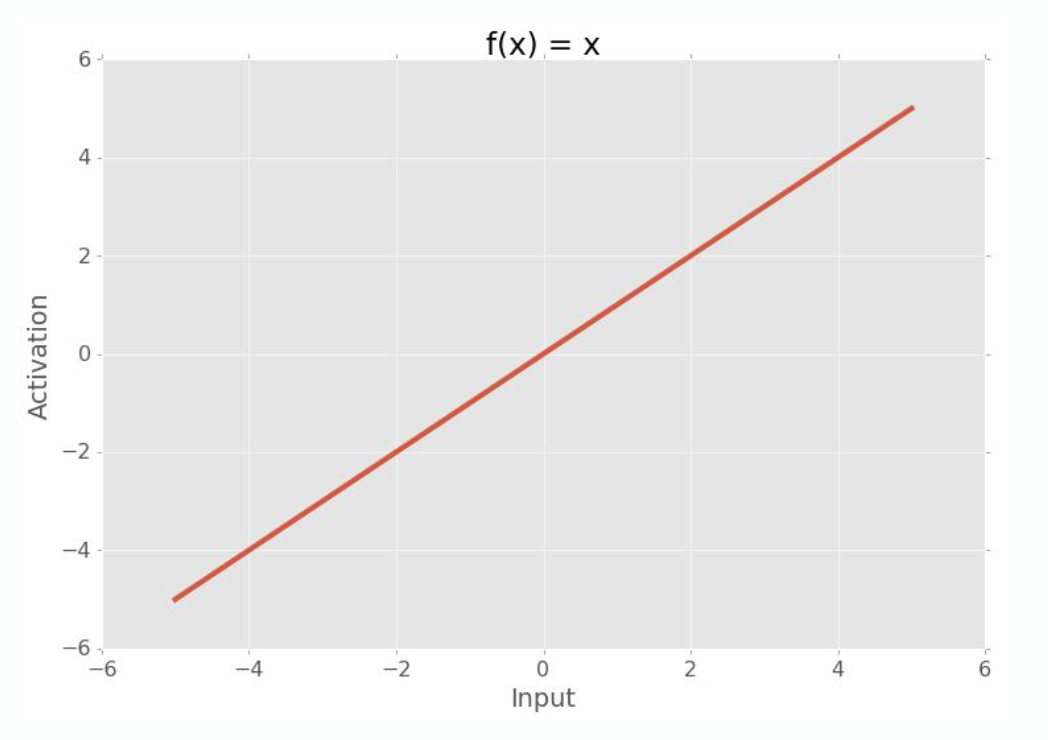
\includegraphics[width=.4\linewidth]{linear_activation.png}
\end{center}

\[ \hat y = h \cdot W_2 = X \cdot W_1 \cdot W_2 = X \cdot A \]

\begin{itemize}
	\item  После линейной активации выход снова линейный
\end{itemize}
\end{frame}


\begin{frame}{От линейной активации ... }
\begin{center}
	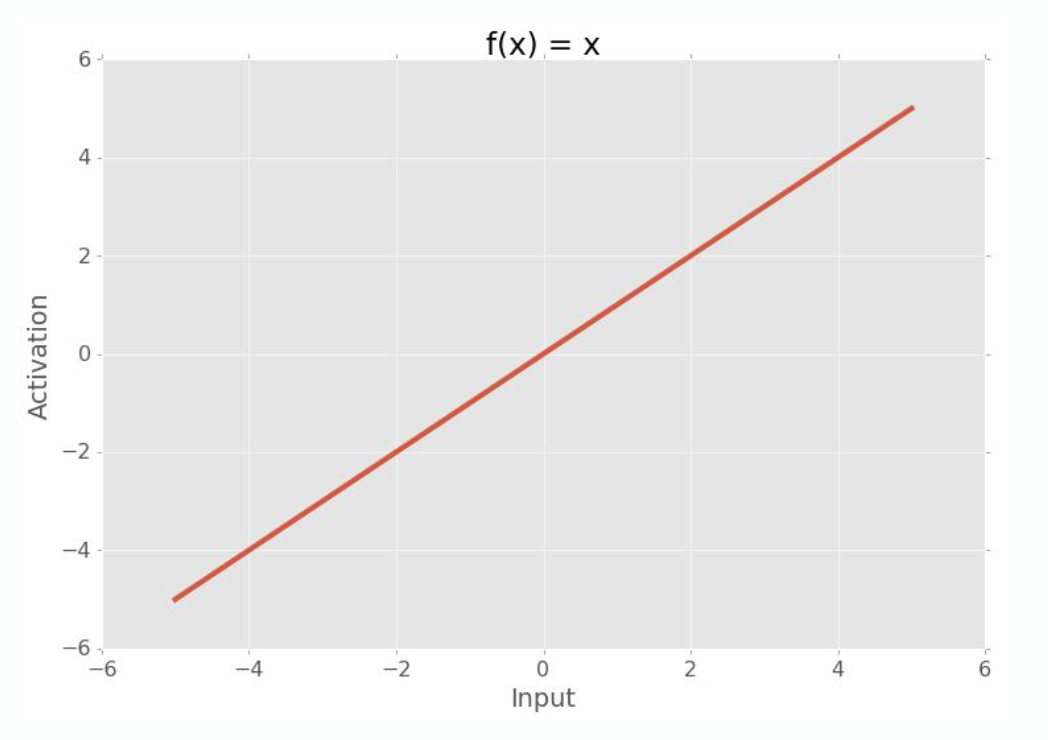
\includegraphics[width=.7\linewidth]{linear_activation.png}
\end{center}
\end{frame}


\begin{frame}{... к нелинейной}
\begin{center}
	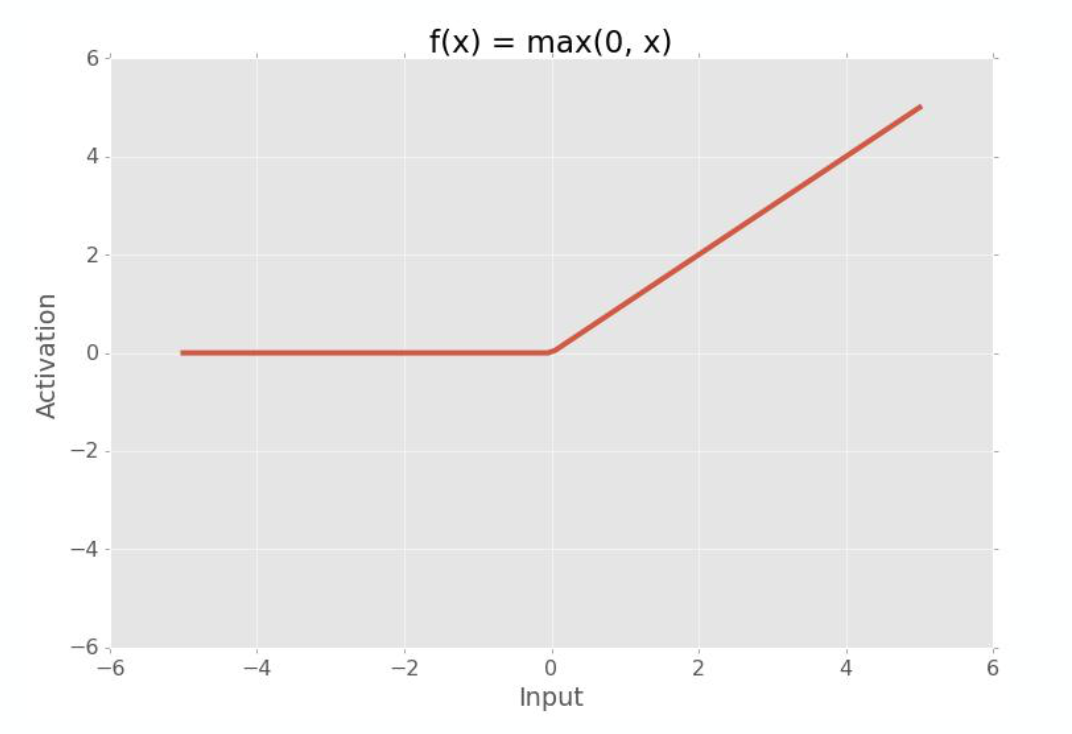
\includegraphics[width=.7\linewidth]{nonlinear_activation.png}
\end{center}
\end{frame}

{
	\usebackgroundtemplate{ 
		\hspace{2cm}
		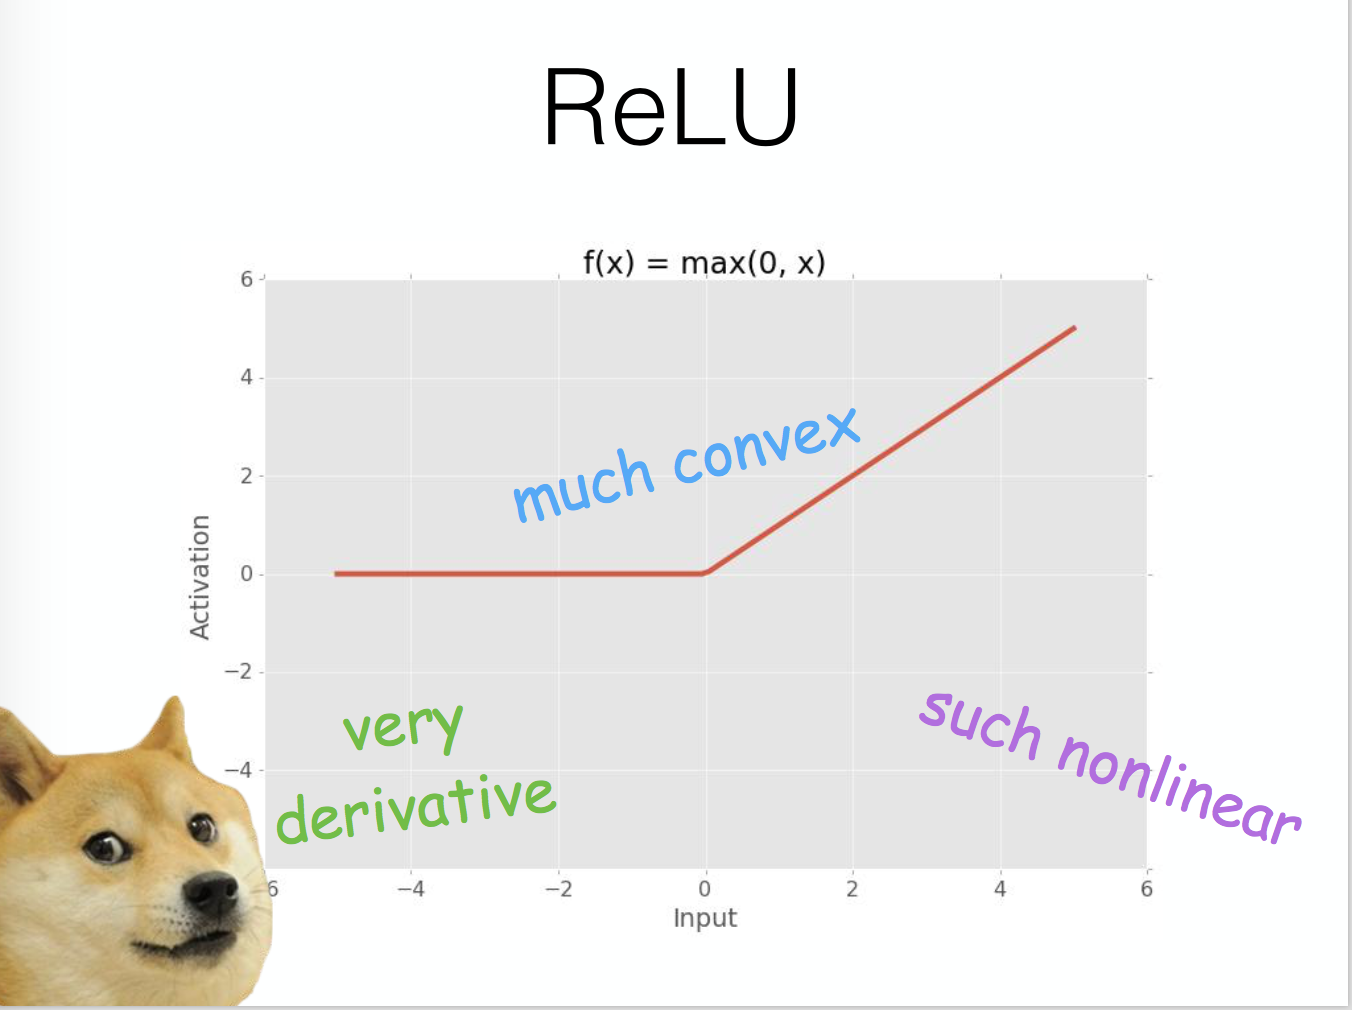
\includegraphics[height=\paperheight]{dogelinear_activation.png}}
\begin{frame}

\end{frame}
}

\begin{frame}{Как обучить перцептрон?}

\[ L(W_1, W_2) =  \frac{1}{2} \cdot (y - f(X \cdot W_1) \cdot W_2)^2\]

Секрет успеха в умении брать производную и градиентном спуске.

\[f(g(x))' = f'(g(x)) \cdot g'(x) \]

\begin{equation*} 
\begin{aligned} 
\frac{\partial L}{\partial W_2} &= - (y - f(X \cdot W_1) \cdot W_2) \cdot f(X \cdot W_1) \\
\frac{\partial L}{\partial W_1} &= - (y - f(X \cdot W_1) \cdot W_2) \cdot W_2 f'(X \cdot W_1) \cdot W_1 
\end{aligned}
\end{equation*}
\end{frame}



\begin{frame}{The Perceptron Convergence Theorem (Rosenblat, 1965)}

\begin{wideitemize}
	\item Любая непрерывная и ограниченная функция может быть сколь угодно точно аппроксимирована нейронной сетью с одним скрытым слоем с нелинейной функцией активации нейрона.
	
	\item Любая функция может быть сколь угодно точно аппроксимирована нейронной сетью с двумя скрытыми слоями с нелинейной функцией активации нейрона.
	
	\item Что ещё можно пожелать?
\end{wideitemize}
\end{frame}

{
\usebackgroundtemplate{ 
	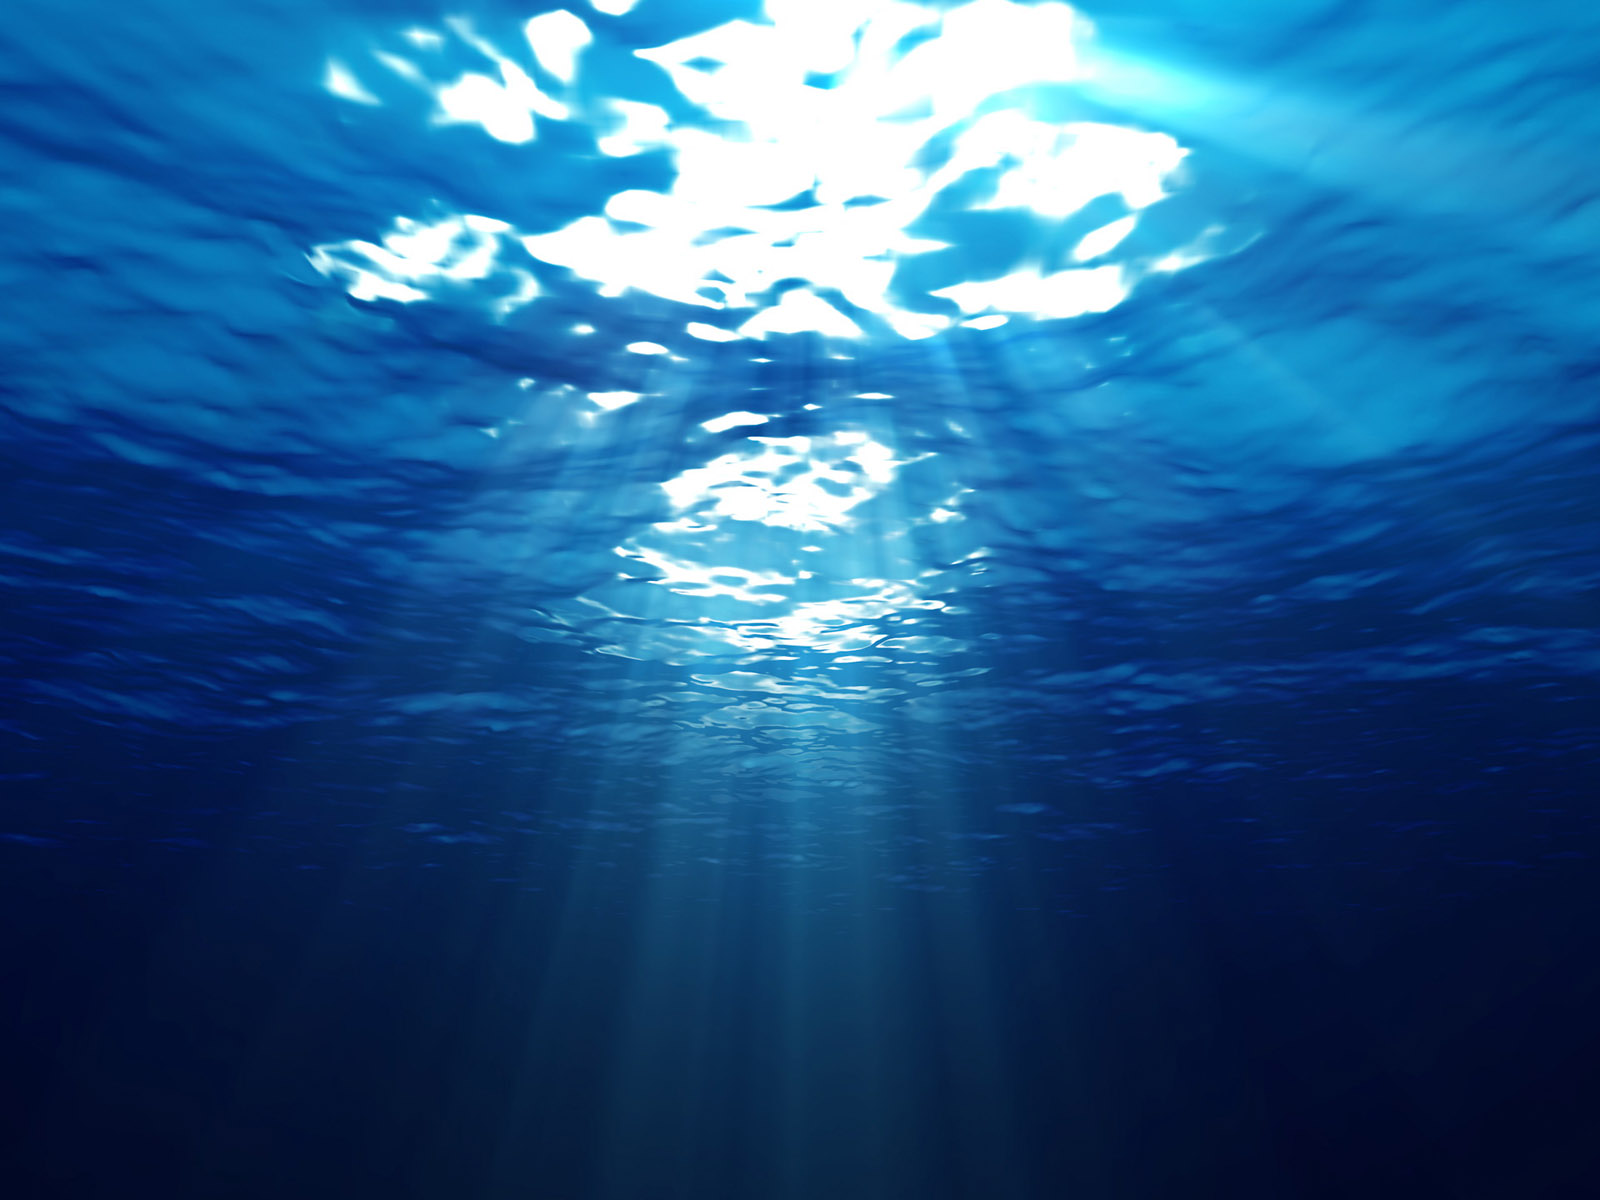
\includegraphics[width=\paperwidth]{goingdeeper.jpg}}
\begin{frame}[fragile]
\vspace{6.5cm}
\begin{center}
{\color{white} \Huge{Going Deeper}}
\end{center}
\end{frame}
}

\begin{frame}{Мотивация}
\begin{wideitemize}
	\item Перцептрон может решить любую проблему, но это дорого
	
	\item Глубокие архитектуры часто позволяют выразить то же самое, приблизить те же функции гораздо более эффективно, чем неглубокие
	
	\item Каждый новый слой сетки будет работать всё с более сложными фичами
\end{wideitemize}

\end{frame}


{
	\usebackgroundtemplate{ 
		\hspace{2cm}
		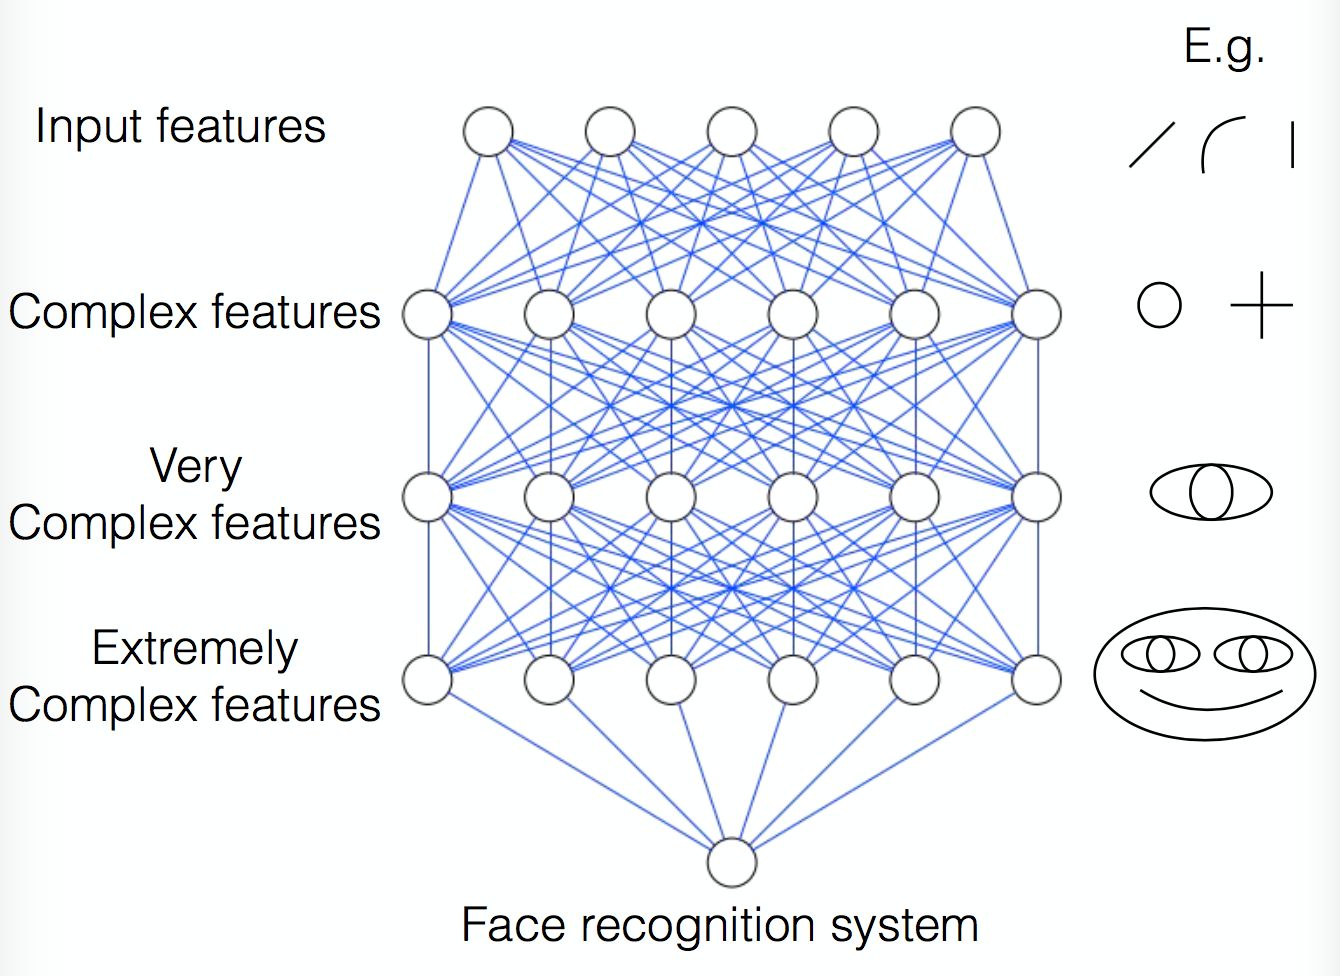
\includegraphics[height=\paperheight]{face.png}}
	\begin{frame}
	
\end{frame}
}


\begin{frame}{Как обучать?}
\begin{wideitemize}
	\item Прямое распространение ошибки (forward propagation): 
	
	\[ X \Rightarrow X \cdot W_1 \Rightarrow f(X \cdot W_1) \Rightarrow f(X \cdot W_1) \cdot W_2 \Rightarrow \ldots \Rightarrow \hat{y} \]
	
	\item Считаем потери:
	
	\[Loss = \frac{1}{2} (y - \hat y)^2\]
	
	\item Ищем производные по цепному правилу ... но это довольно дорого
	
	\item До определённого момента люди не знали как легко обучать нейросети
\end{wideitemize}
\end{frame}


\begin{frame}{Backpropogation}
\begin{center}
	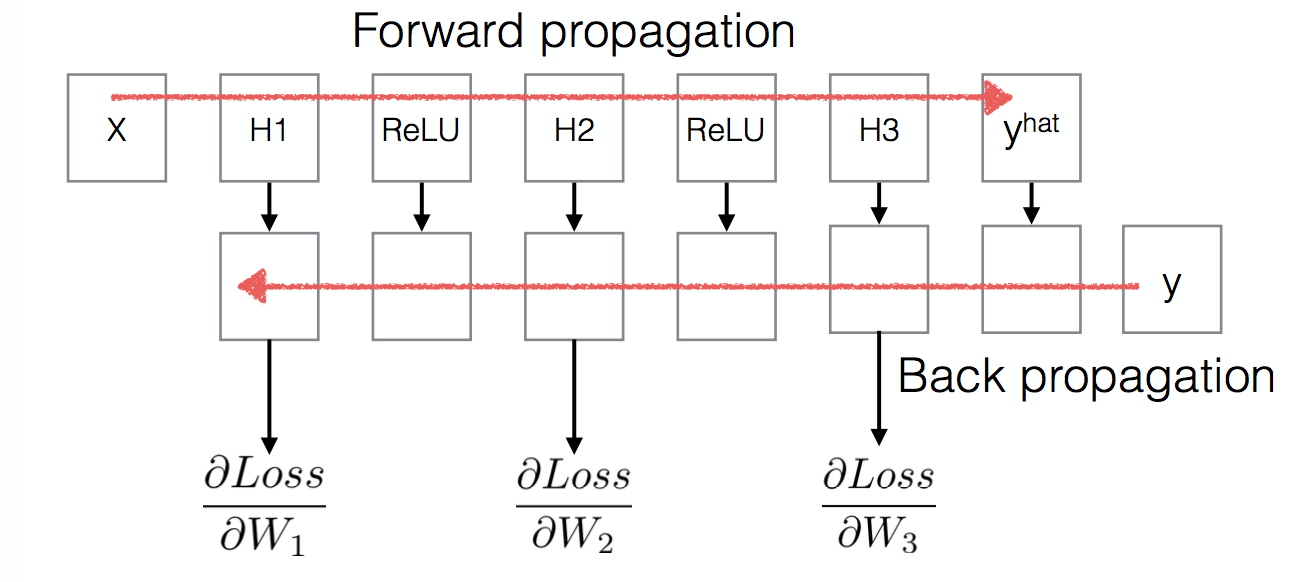
\includegraphics[width=.8\linewidth]{backpropagation.png}
\end{center}
\end{frame}


\begin{frame}{Lego}
\begin{center}
	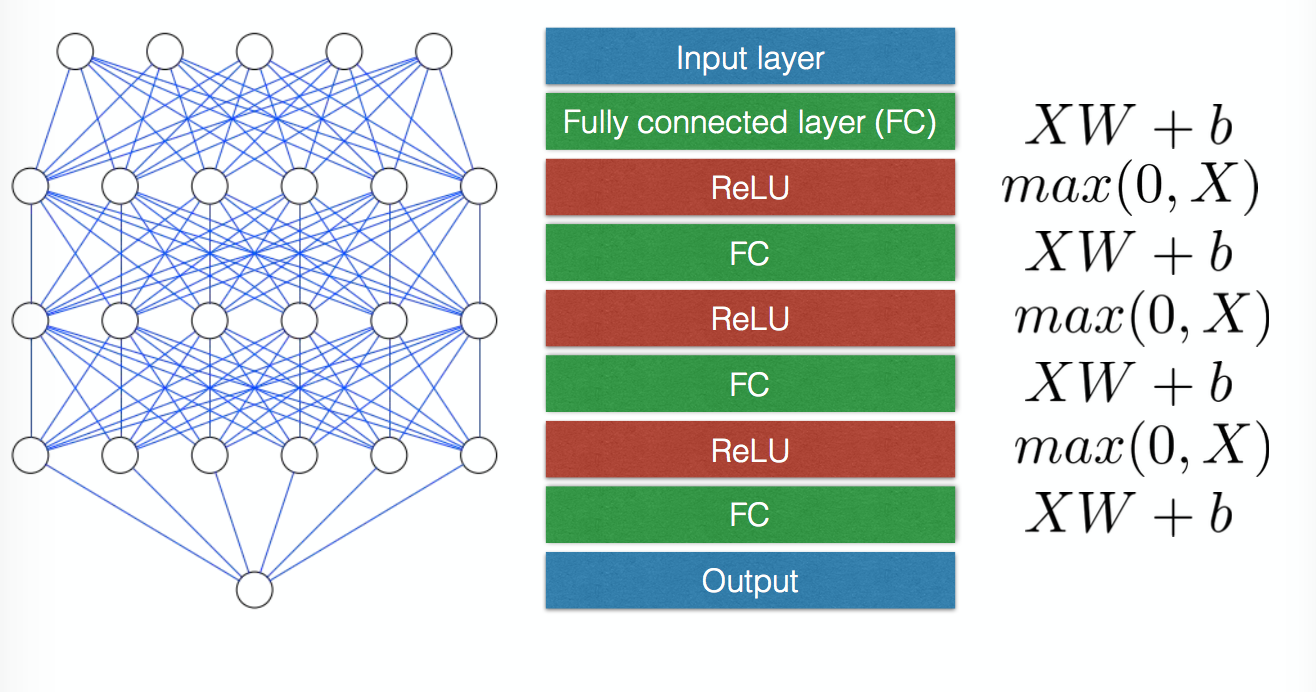
\includegraphics[width=.99\linewidth]{lego.png}
\end{center}
\end{frame}


\begin{transitionframe}
	\begin{center}
		\Huge Учим нейросеть руками!
	\end{center}
\end{transitionframe}

\end{document}
